\documentclass[a4j]{jbook}
\usepackage[dvipdfm]{graphicx}
\usepackage{here}
\usepackage{color}
\usepackage{ascmac}	
\usepackage{framed}
\renewcommand{\bibname}{参考文献}
\title{UDASインストールマニュアル}
\author{IUGONETプロジェクト\\iugonet@www.iugonet.org}
\date{\today}
\begin{document}
\maketitle
\tableofcontents

\part{UDAS概要}
\label{udas_abstract}
\chapter{UDASとは?}
\label{whats_udas}

IUGONETデータ解析ソフトウェア(UDAS: iUgonet Data Analysis Software)は、
IUGONETプロジェクト参加機関が公開している超高層大気分野の様々な地上観測データを
プロット・解析する為のソフトウェアです。例えば、
京大地磁気センターが公開しているAE指数(図\ref{ae})、
国立極地研究所が公開しているEISCATレーダーのデータ(図\ref{eiscat})、
名大STE研が公開しているSuperDARN北海道レーダーの
データ(図\ref{superdarn})等をプロット・解析することが可能です。
\begin{figure}[H]
\begin{center}
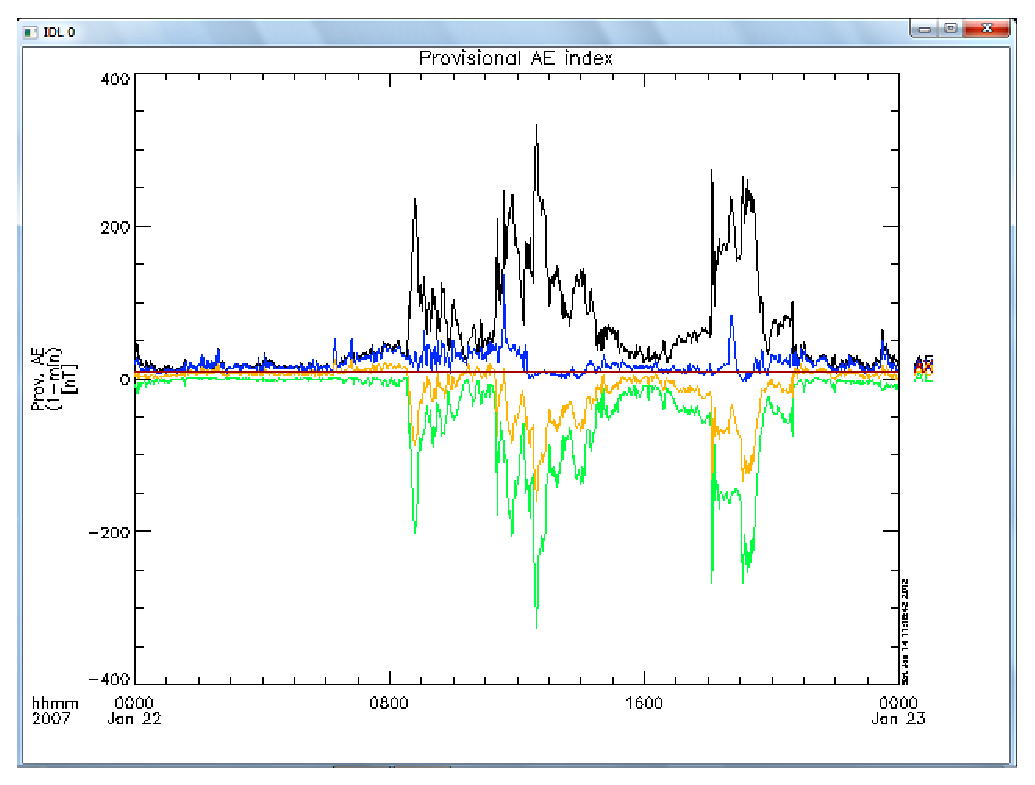
\includegraphics[width=10cm]{images/screenshot_iug_crib_gmag_wdc.eps}
\caption{UDASを用いたAE指数のプロット。}
\label{ae}
\end{center}
\end{figure}

\begin{figure}[H]
\begin{center}
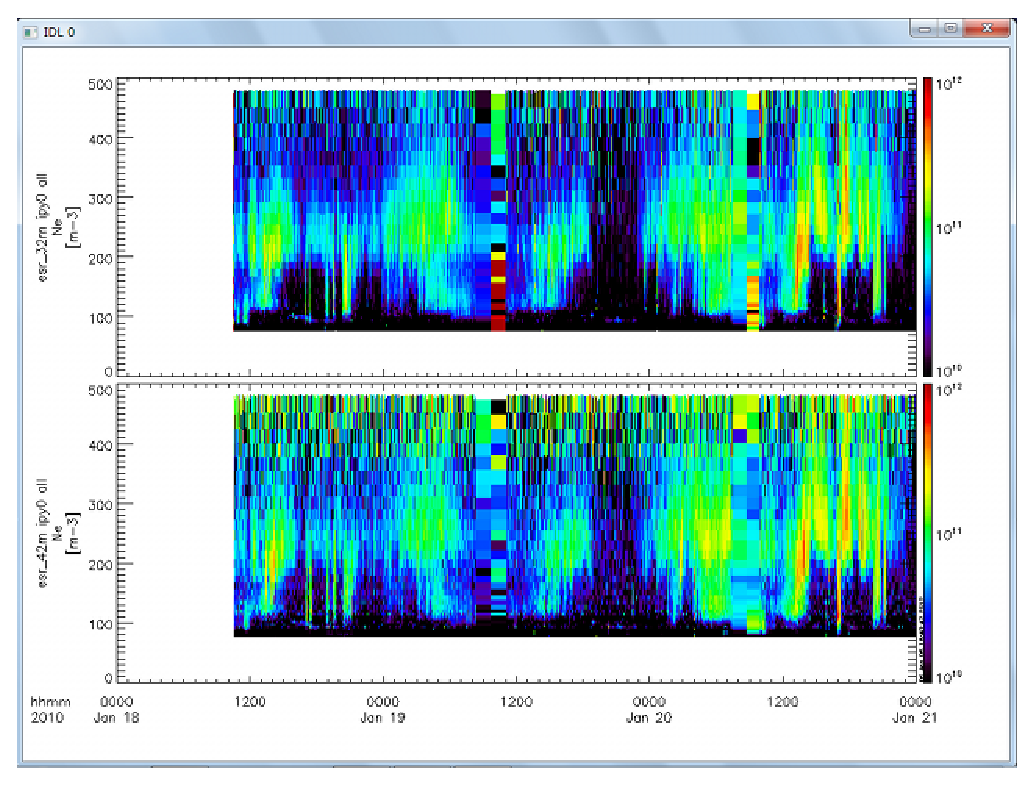
\includegraphics[width=10cm]{images/screenshot_iug_crib_eiscat.eps}
\caption{UDASを用いたEISCATレーダーデータのプロット。}
\label{eiscat}
\end{center}
\end{figure}

\begin{figure}[H]
\begin{center}
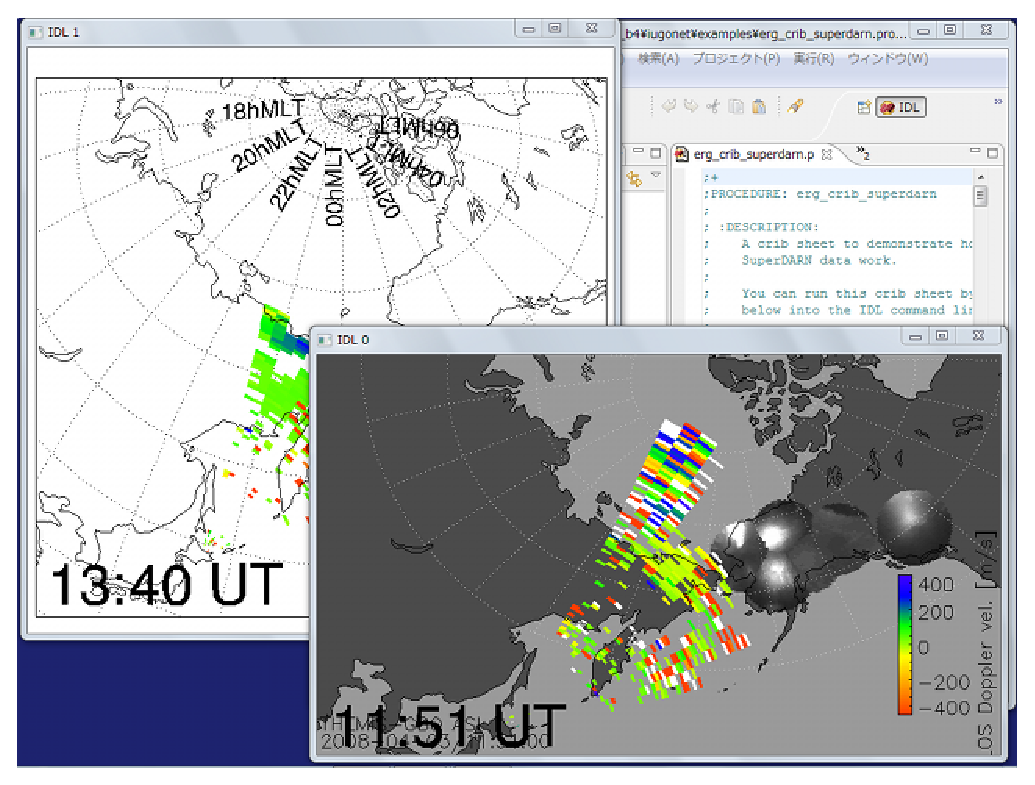
\includegraphics[width=10cm]{images/screenshot_erg_crib_superdarn.eps}
\caption{UDASを用いたSuperDARN北海道レーダーデータのプロット。}
\label{superdarn}
\end{center}
\end{figure}

\chapter{UDASの構成}
UDAS は、独立した1つのソフトウェアでなく、その多くの機能は
THEMIS Data Analysis Software suite (TDAS)と呼ばれる
THEMIS衛星データ等\footnote{TDASは、THEMIS以外にも、GOES、WIND、ACEのデータを扱うことが出来ます。}のデータを解析する為のソフトウェアの機能を利用しています。
そして、このTDASは商用ソフトウェアであるIDL上で動くソフトウェアです。つまり、UDASは
TDASならびにIDLに依存していると言えます(図\ref{udas_deploy})。
\begin{figure}[H]
\begin{center}
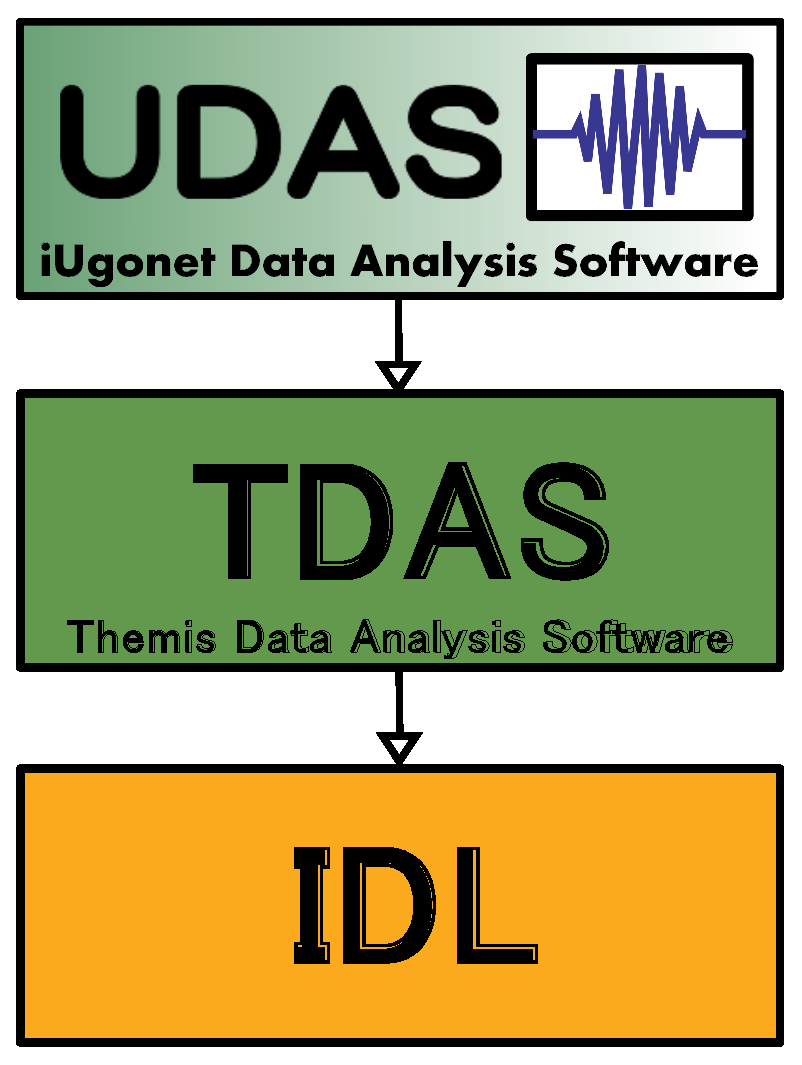
\includegraphics[width=2.5cm]{images/udas_deploy.eps}
\caption{IDL-TDAS-UDASの関係図。UDASはTDASに依存し、TDASはIDLに依存しています。}
\label{udas_deploy}
\end{center}
\end{figure}
%(図\ref{udas_installation_workflow})。
%\begin{figure}[H]
%\begin{center}
%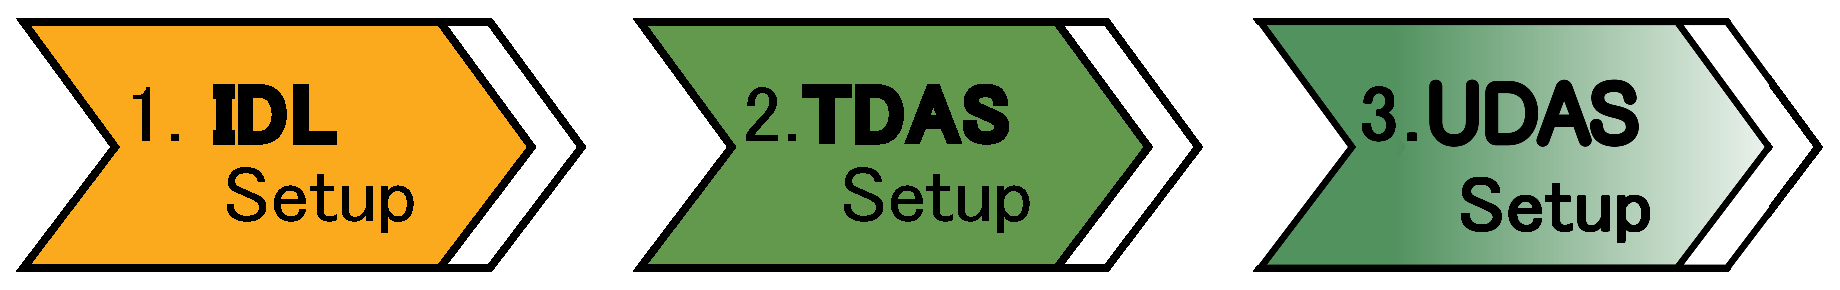
\includegraphics[width=10cm]{images/udas_installation_workflow.eps}
%\caption{IDL-TDAS-UDASのインストールの流れ。}
%\label{udas_installation_workflow}
%\end{center}
%\end{figure}
本インストールマニュアルは、
\today 現在において最新のUDAS 1.00のインストール方法を
解説します\footnote{
TDAS 5.21ベースであるUDAS 0.21b1を利用することも可能ですが、
既にこのバージョンの開発は終了しています。そして、サポートされている
ロードプロシージャも少ないので、最新版のUDASを利用することを
オススメします。TDAS 5.21とUDAS 0.21b1をインストールする場合は、
両ソフトウェアのバージョン番号を適宜読み替えて、本インストール
マニュアルをご覧下さい。}。
この為、UDASのインストールに先立って、IDLとTDASのインストールが必要になりますが、
本書は、TDASとUDASのインストールのみ記載しています。IDLのインストールが未だの方は、
先にIDLをインストールした後に、本書をお読み下さい。

それでは、各OS毎にTDAS/UDASのインストール方法を説明しますので、
Windowsユーザーの方は第\ref{tdas_install_windows}章、
Linuxユーザーの方は第\ref{tdas_install_linux}章、
Macユーザーの方は第\ref{tdas_install_mac}章、
へ進んで下さい。

\part{TDAS/UDASのインストール(Windows編)}
\chapter{TDASのインストール(Windows編)}
\label{tdas_install_windows}
第\ref{udas_abstract}章の図\ref{udas_deploy}に示したように、
TDASはIDL上で動作する為、TDASのインストールに先立って、IDLのインストールが必要です。
IDL6.3$\sim$7.1が既にインストールされていることを確認した上で、本章を読み進めて下さい。

\section{TDASのダウンロード}
最初に、tdas\_6\_00.zipをユーザーのダウンロードフォルダーにダウンロードします。
\begin{screen}
\begin{verbatim}
http://themis.ssl.berkeley.edu/socware/tdas_6_00/tdas_6_00.zip
\end{verbatim}
\end{screen}
Internet Explorer等のブラウザを用いて上記URLにアクセスしてダウンロードして下さい\footnote{ネットワーク
環境によって、proxyサーバーの設定が必要な場合があります。}。

\section{TDASの展開}
次に、ホームディレクトリ上において、tdas\_6\_00.zipを展開します。
正しく展開出来ていれば、ホームディレクトリにtdas\_6\_00ディレクトリが出来ます。

\section{TDASの環境設定1(パスの設定)}

\subsection{IDLDE 7.0/7.1}

\subsubsection{IDL Workbenchの起動}

\includegraphics[width=0.5cm]{images/windows_start_button.eps}([スタート]ボタン)$\rightarrow$すべてのプログラム$\rightarrow$[IDL 7.1]$\rightarrow$[IDL Workbench]\\
でIDL Workbenchを起動します。

\subsubsection{設定}
[ウィンドウ(W)]$\rightarrow$[設定(P)...]$\rightarrow$[IDL]$\rightarrow$[パス]$\rightarrow$[挿入...]$\rightarrow$
"ディレクトリを選択"によってウィンドウが開くので、
展開したディレクトリ(tdas\_6\_00)を選択$\rightarrow$
選択したディレクトリが設定ウィンドウに表示されるので左側のチェックボックスをチェック$\rightarrow$[OK]\\
を行います。

\subsection{IDLDE 6.4以前}
\subsubsection{IDLの起動}

\includegraphics[width=0.5cm]{images/windows_start_button.eps}([スタート]ボタン)$\rightarrow$
すべてのプログラム$\rightarrow$[IDL 6.4]$\rightarrow$IDL\\
でIDLを起動します。\\
File$\rightarrow$Preferences$\rightarrow$Path$\rightarrow$Insert$\rightarrow$展開したディレクトリ(tdas\_6\_00)を選択$\rightarrow$
選択したディレクトリが表示されるので左側のチェックボックスをチェック$\rightarrow$OK\\
を行います。

\section{TDASの動作確認}
IDLを起動し、thm\_initコマンドを入力し、以下のメッセージが出れば、無事にパスが通っています。
\begin{screen}
\begin{verbatim}
IDL> thm_init [enter]
THEMIS countdown: xxxxxx xxxxxx xxxx since launch
THEMIS>  
\end{verbatim}
\end{screen}

\section{TDASの環境設定2(Local data directoryとRemote data directoryの設定)}
 TDASで、Local data directoryとRemote data directoryの設定を行います。
まず始めに、IDLを起動してthm\_gui\_newコマンドを入力します。
\begin{screen}
\begin{verbatim}
   IDL> thm_gui_new
\end{verbatim}
\end{screen}
次に、\fbox{File}$\rightarrow$\fbox{Configuration Settings...}を選択します。
Configuration Settings... で、THEMIS を選択します。\par
ダウンロードされたTHEMISデータを保存するディレクトリであるLocal data directory
を設定します。ここでは、ユーザーのホームディレクトリ/data/themisに設定します。\par
最後に、ダウンロード元であるRemote data directoryを設定します。日本国内でTDASを
使用する場合、日本のミラーサイトであり、ネットワーク的に近い
http://themis.stp.isas.jaxa.jp/data/themis/
を設定します。
\fbox{Save}-\fbox{Close}をクリックします。

\chapter{UDASのインストール(Windows編)}
\label{udas_install_windows}

第\ref{udas_abstract}章の図\ref{udas_deploy}で示したように、UDASはTDASに依存しています。その為、
UDASのインストールに先立ち、TDASのインストールが必要です。TDASを未だインストールされて
いない場合は、先に第\ref{tdas_install_windows}章をご覧下さい。

\section{UDASのダウンロード}
最初に、udas\_1\_00\_1.zipをユーザーのダウンロードフォルダーにダウンロードします。
\begin{screen}
\begin{verbatim}
http://www.iugonet.org/software/udas_package_j/udas_1_00_1.zip
\end{verbatim}
\end{screen}
Internet Explorer等のブラウザを用いて上記URLにアクセスしてダウンロードして下さい。

\section{UDASの展開}
次にホームディレクトリ上において、udas\_1\_00\_1.zipを展開します。
正しく展開出来ていれば、ホームディレクトリにudas\_1\_00\_1ディレクトリが出来ます。
\section{UDASの環境設定}

\subsection{IDLDE 7.0/7.1}

\begin{enumerate}
\item IDLを起動します。
\item \fbox{\underline{W}indow}メニューから\fbox{\underline{P}references}を選択します(図\ref{idl71/Fig2.eps})。
\item Preferencesウィンドウが開くので、"IDL"$\rightarrow$"Paths"を選択します(図\ref{idl71/Fig3.eps})。
\item \fbox{Insert...} をクリックします(図\ref{idl71/Fig3.eps})。
\item ダウンロードして展開したUDASディレクトリを選択し、OK をクリックします(図\ref{idl71/Fig8.eps})。
\item 表示されたtdas\_6\_00ディレクトリの左にあるチェックボックスにチェックを入れます(図\ref{idl71/Fig5.eps})。
\item 右側にある Move up ボタンを押して、UDAS ディレクトリを TDAS ディレクトリの上に持っていく(図\ref{idl71/Fig5.eps})。
\item \fbox{OK}をクリック(図\ref{idl71/Fig5.eps})。
\item IDLコマンドラインで、.full\_reset\_session  を実行します。(図\ref{idl71/Fig6.eps})
\end{enumerate}

%\begin{figure}[H]
%\begin{center}
%\includegraphics[width=9cm]{images/fig_idl71/Fig1.eps}
%\caption{idl71/Fig1.eps}
%\label{idl71Fig1.eps}
%\end{center}
%\end{figure}

\begin{figure}[H]
\begin{center}
\includegraphics[width=9cm]{images/fig_idl71/Fig2.eps}
\caption{IDL Workbench (Windows, IDL71)}
\label{idl71/Fig2.eps}
\end{center}
\end{figure}

\begin{figure}[H]
\begin{center}
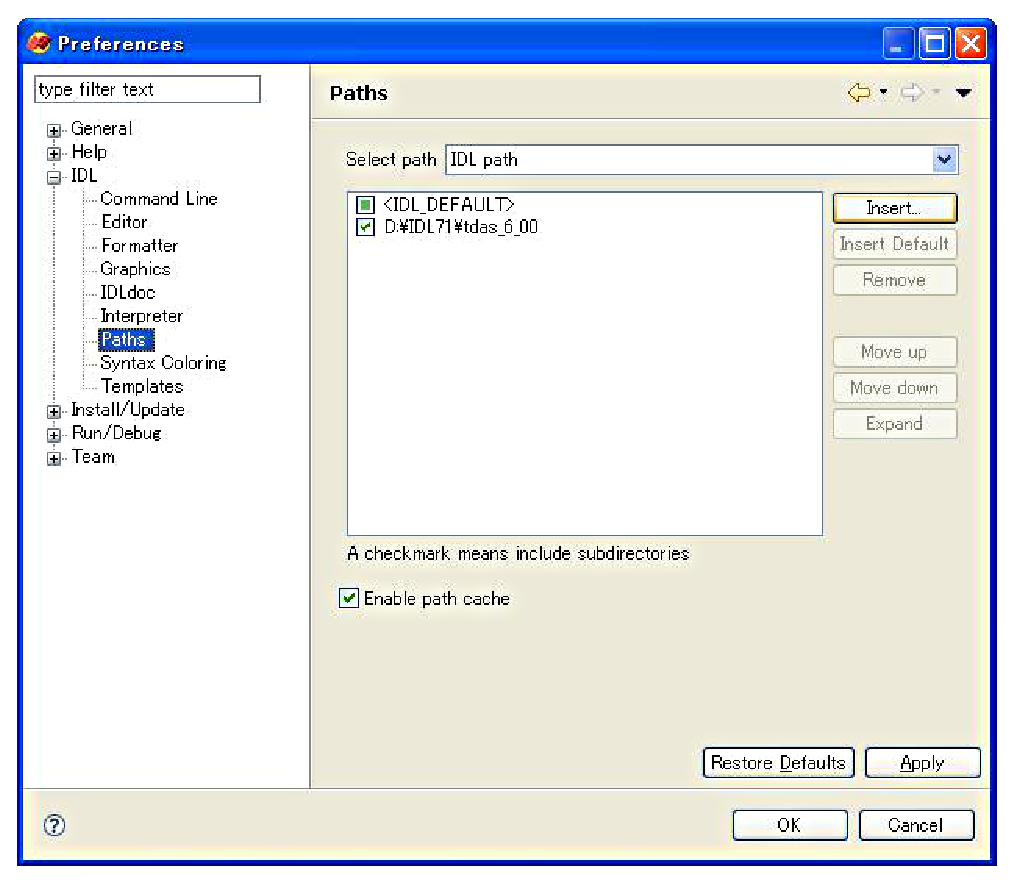
\includegraphics[width=9cm]{images/fig_idl71/Fig3.eps}
\caption{Preferences (Windows, IDL71)}
\label{idl71/Fig3.eps}
\end{center}
\end{figure}

\begin{figure}[H]
\begin{center}
\includegraphics[width=9cm]{images/fig_idl71/Fig8.eps}
\caption{Select Directory (Windows, IDL71)}
\label{idl71/Fig8.eps}
\end{center}
\end{figure}

\begin{figure}[H]
\begin{center}
\includegraphics[width=9cm]{images/fig_idl71/Fig5.eps}
\caption{Preferences (Windows, IDL71)}
\label{idl71/Fig5.eps}
\end{center}
\end{figure}

\begin{figure}[H]
\begin{center}
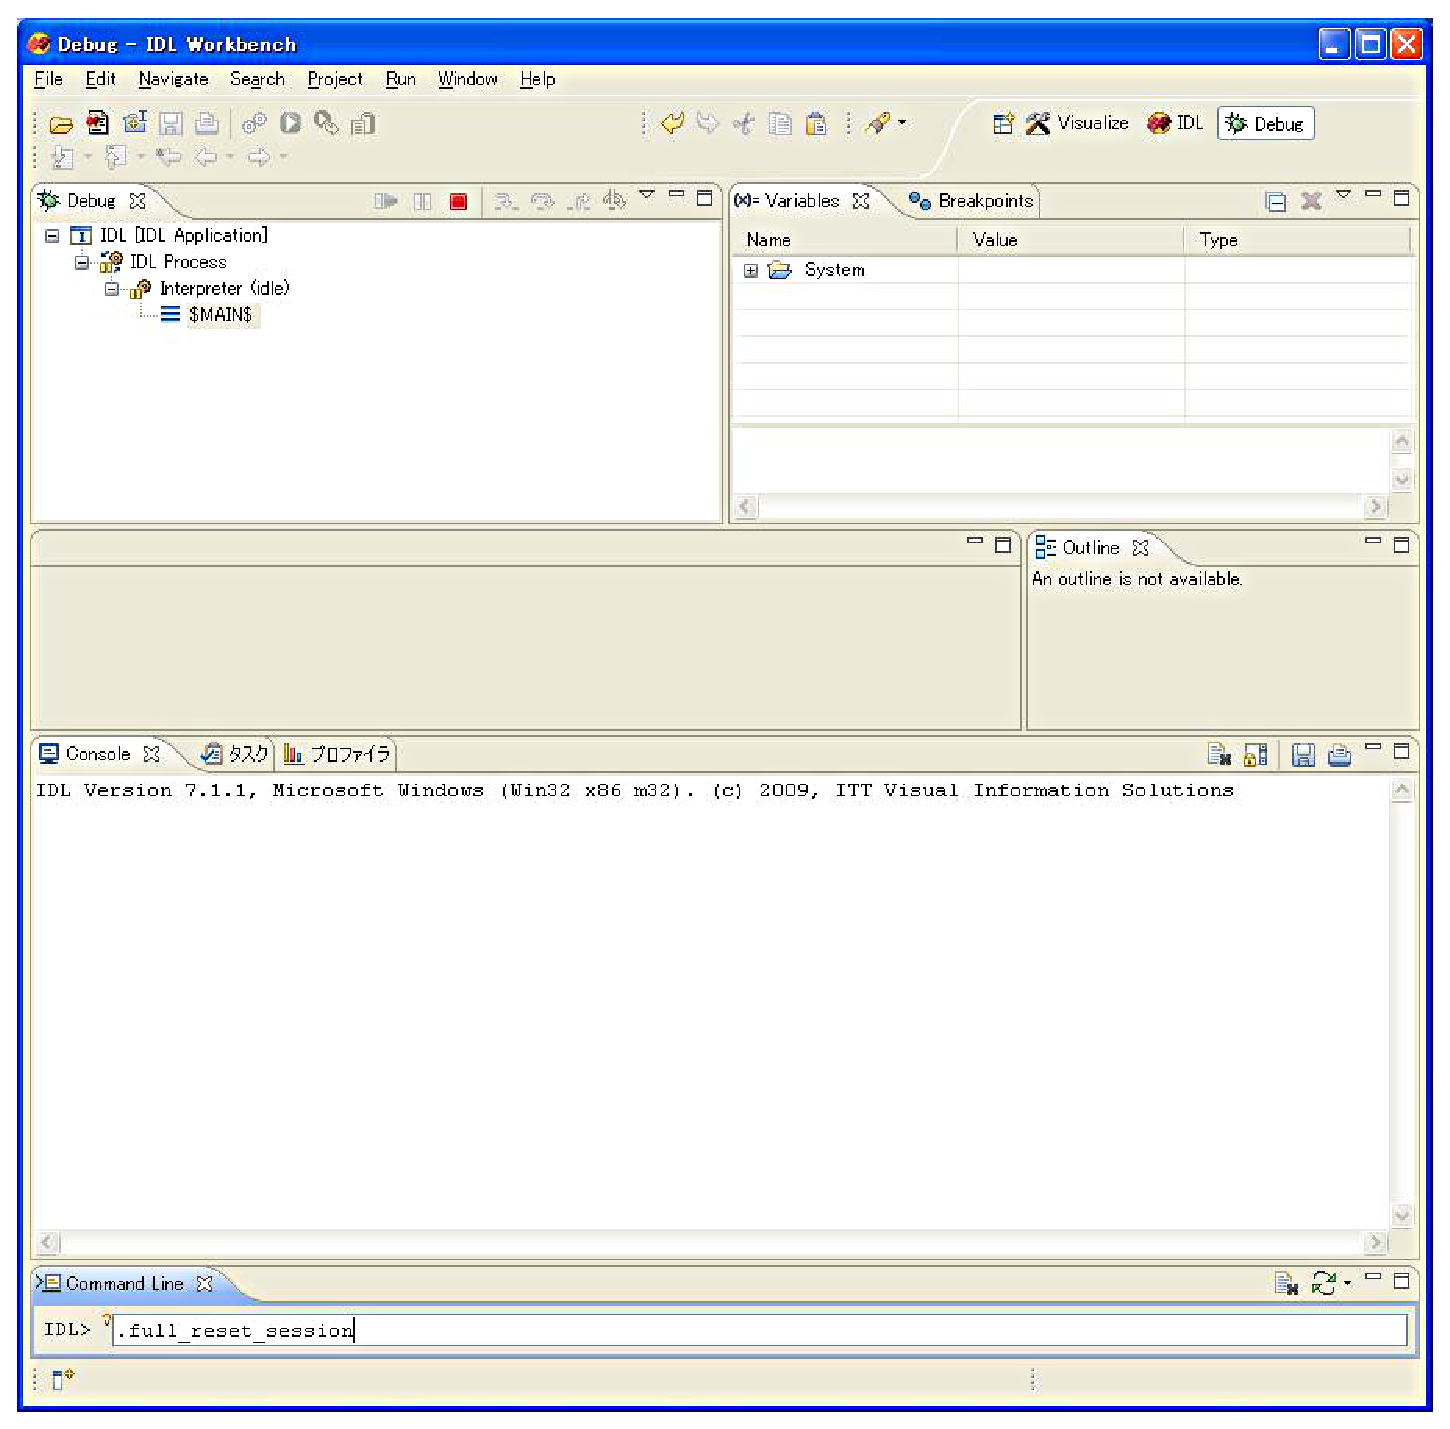
\includegraphics[width=9cm]{images/fig_idl71/Fig6.eps}
\caption{IDL Workbench (Windows, IDL71)}
\label{idl71/Fig6.eps}
\end{center}
\end{figure}

%\begin{figure}[H]
%\begin{center}
%\includegraphics[width=9cm]{images/fig_idl71/Fig7.eps}
%\caption{Preferences (Windows, IDL71)}
%\label{idl71/Fig7.eps}
%\end{center}
%\end{figure}

\subsection{IDLDE 6.4  以前のバージョン:}
\begin{enumerate}
\item IDLを起動します。
\item \fbox{\underline{F}ile}メニューから\fbox{\underline{P}references}を選択します(図\ref{idl64/Fig2.eps})。
\item Pathタブを選択(図\ref{idl64/Fig3.eps})。
\item \fbox{\underline{I}nsert}をクリックします(図\ref{idl64/Fig3.eps})。
\item ダウンロードして展開したUDASディレクトリを選択し、\fbox{OK}をクリックします(図\ref{idl7164/Fig8.eps})。
\item 作成されたディレクトリの左にあるチェックボックスにチェックを入れます(図\ref{idl64/Fig5.eps})。
\item 右側にある上向き矢印を押して、UDAS ディレクトリを TDAS ディレクトリの上に持っていきます(図\ref{idl64/Fig5.eps})。
\item \fbox{OK}をクリックします(図\ref{idl64/Fig5.eps})。
\item IDLコマンドラインで、.full\_reset\_sessionを実行します(図\ref{idl64/Fig6.eps})。
\end{enumerate}

%\begin{figure}[H]
%\begin{center}
%\includegraphics[width=9cm]{images/fig_idl64/Fig1.eps}
%\caption{idl64/Fig1.eps}
%\label{idl64/Fig1.eps}
%\end{center}
%\end{figure}

\begin{figure}[H]
\begin{center}
\includegraphics[width=9cm]{images/fig_idl64/Fig2.eps}
\caption{IDL Workbench (Windows, IDL64)}
\label{idl64/Fig2.eps}
\end{center}
\end{figure}

\begin{figure}[H]
\begin{center}
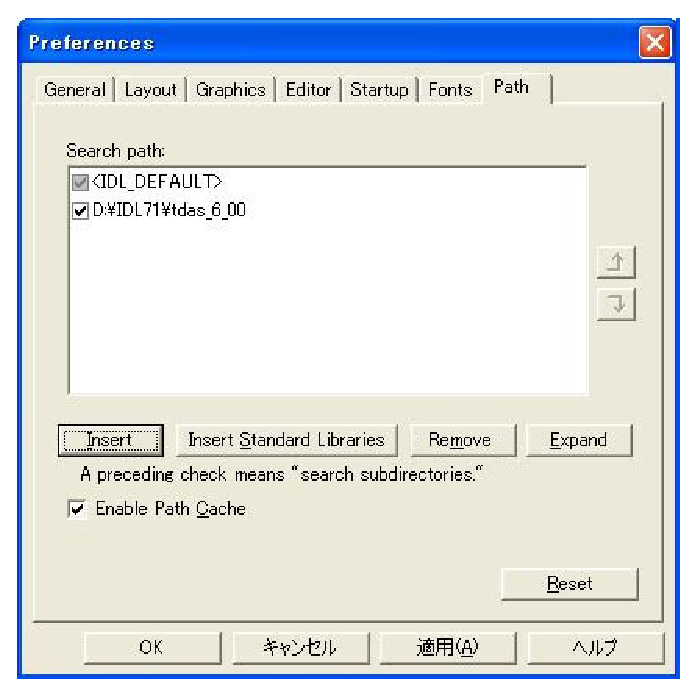
\includegraphics[width=9cm]{images/fig_idl64/Fig3.eps}
\caption{Preferences (Windows, IDL64)}
\label{idl64/Fig3.eps}
\end{center}
\end{figure}

\begin{figure}[H]
\begin{center}
\includegraphics[width=9cm]{images/fig_idl71/Fig8.eps}
\caption{Select Directory (Windows, IDL64)}
\label{idl7164/Fig8.eps}
\end{center}
\end{figure}

%\begin{figure}[H]
%\begin{center}
%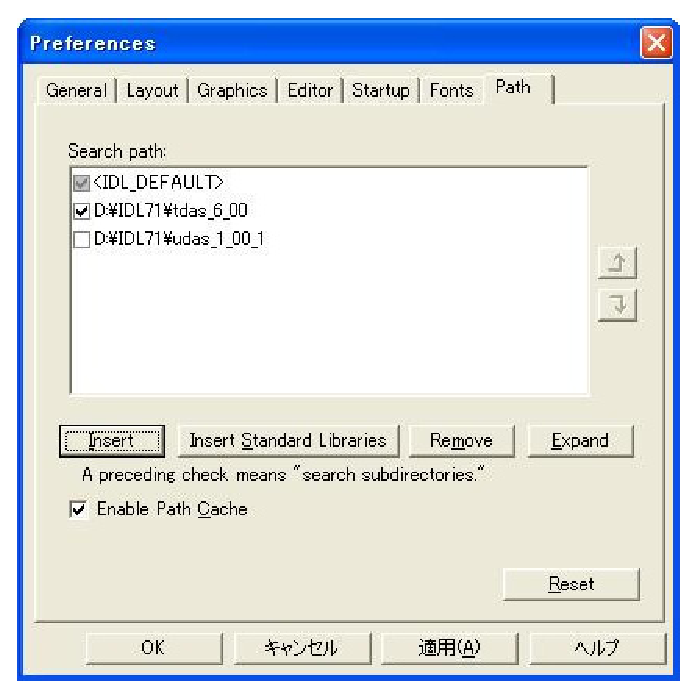
\includegraphics[width=9cm]{images/fig_idl64/Fig4.eps}
%\caption{Preferences (Windows, IDL64)}
%\label{idl64/Fig4.eps}
%\end{center}
%\end{figure}

\begin{figure}[H]
\begin{center}
\includegraphics[width=9cm]{images/fig_idl64/Fig5.eps}
\caption{Preferences (Windows, IDL64)}
\label{idl64/Fig5.eps}
\end{center}
\end{figure}

\begin{figure}[H]
\begin{center}
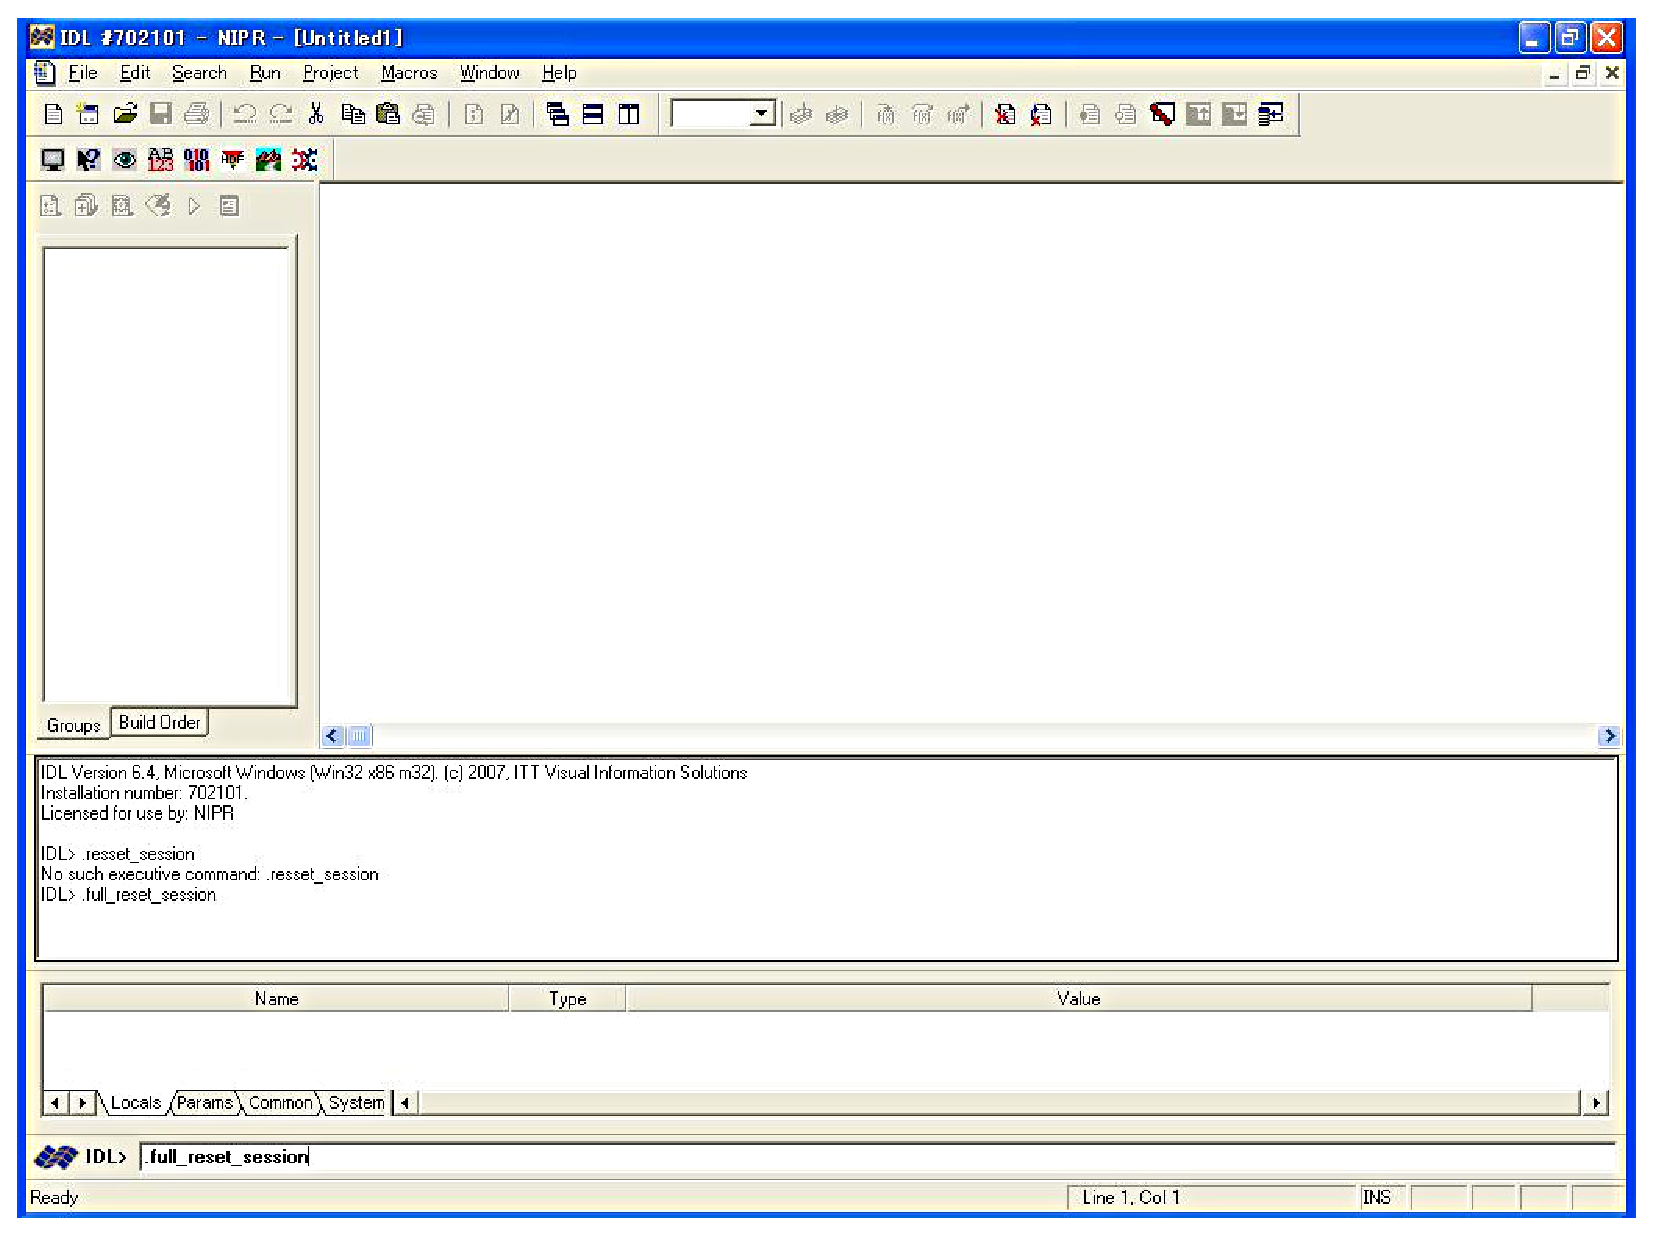
\includegraphics[width=9cm]{images/fig_idl64/Fig6.eps}
\caption{IDL Workbench (Windows, IDL64)}
\label{idl64/Fig6.eps}
\end{center}
\end{figure}

\section{UDASの動作確認}
ここでは、UDASのGUIの動作確認を行います。まず始めに、
IDLを起動して、下記コマンドを入力します。
\begin{screen}
\begin{verbatim}
   IDL> thm_gui_new
\end{verbatim}
\end{screen}
THEMIS Main Windowが開いた後に、\fbox{File}-\fbox{Load Data}を選択します(図\ref{idl64/Fig8.eps})。
新しく開いたウィンドウにIUGONETタブがあれば動作確認終了です。(図\ref{thm_gui_windows2.eps})
%\begin{figure}[H]
%\begin{center}
%\includegraphics[width=9cm]{images/fig_idl64/Fig7.eps}
%\caption{IDL Workbench (Windows, IDL64)}
%\label{idl64/Fig7.eps}
%\end{center}
%\end{figure}

\begin{figure}[H]
\begin{center}
\includegraphics[width=9cm]{images/fig_idl64/Fig8.eps}
\caption{THEMIS: Main Window (Windows, IDL64)}
\label{idl64/Fig8.eps}
\end{center}
\end{figure}

\begin{figure}[H]
\begin{center}
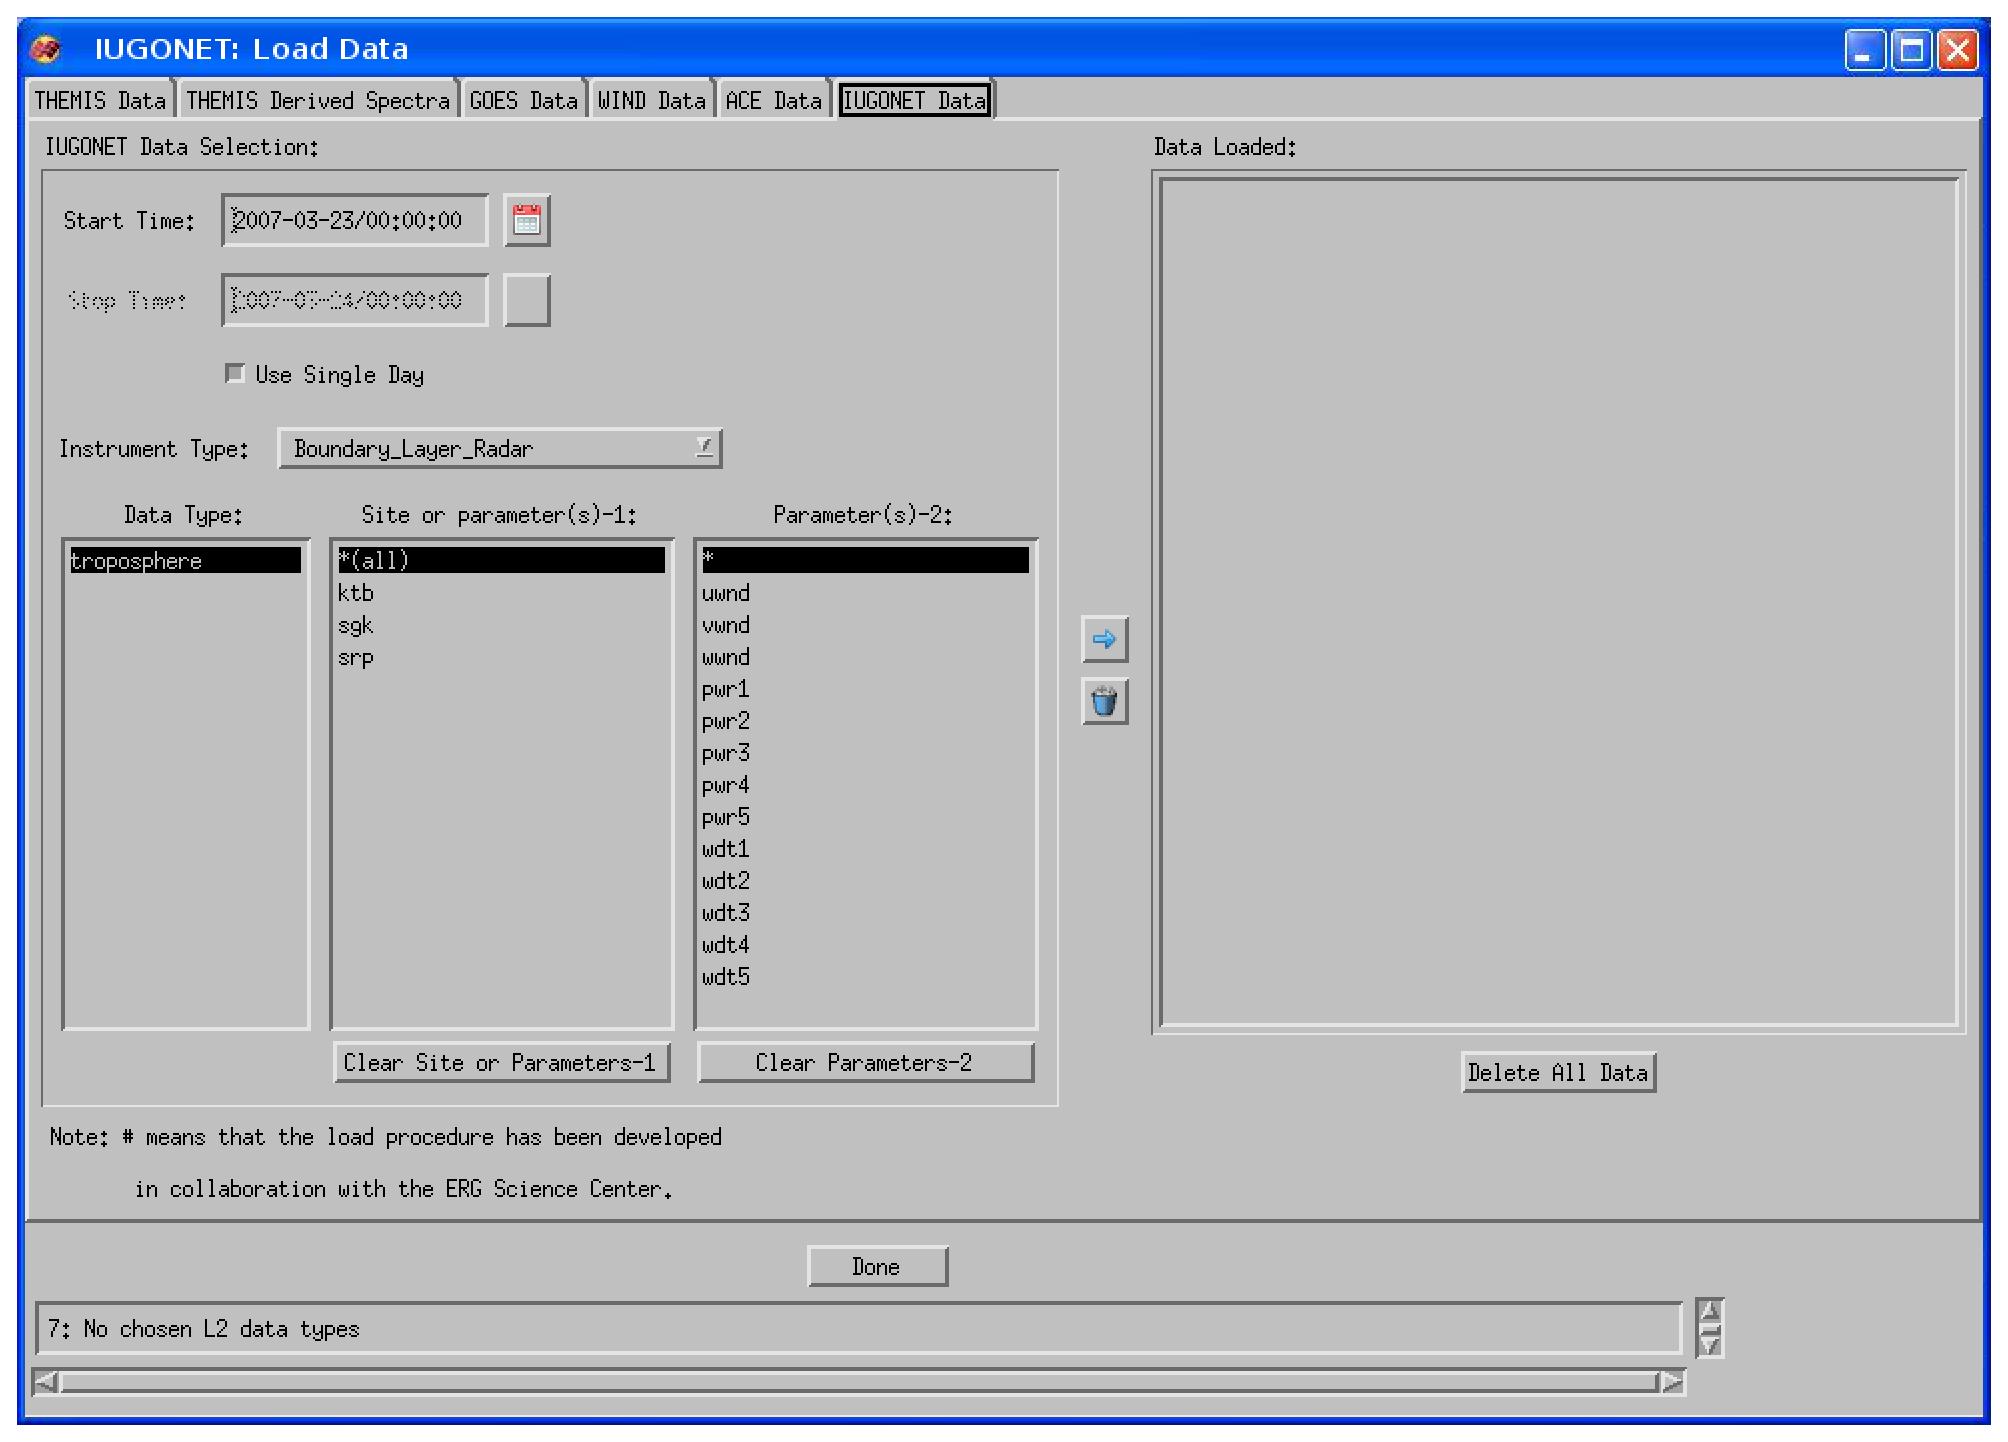
\includegraphics[width=9cm]{images/thm_gui_windows2.eps}
\caption{IUGONET: Load Data (Windows)}
\label{thm_gui_windows2.eps}
\end{center}
\end{figure}

\part{TDAS/UDASのインストール(Linux編)}

\chapter{TDASのインストール(Linux編)}
\label{tdas_install_linux}

第\ref{udas_abstract}章の図\ref{udas_deploy}に示したとおり、
TDASはIDL上で動作する為、TDASのインストールに先立って、IDLのインストールが必要です。
IDL6.3$\sim$7.1が既にインストールされていることを確認した上で、本章を読み進めて下さい。

\section{TDASのダウンロード}
最初に、tdas\_6\_00.zipをユーザーのホームディレクトリにダウンロードします。
\begin{screen}
\begin{verbatim}
   $ wget http://themis.ssl.berkeley.edu/socware/tdas_6_00/tdas_6_00.zip
\end{verbatim}
\end{screen}
もしくは
\begin{screen}
\begin{verbatim}
   $ curl http://themis.ssl.berkeley.edu/socware/tdas_6_00/tdas_6_00.zip 
\end{verbatim}
\end{screen}
を実行します。上記のコマンドでUDASがダウンロード出来ない
場合は、Firefox等のブラウザを用いて上記URLにアクセスしてダウンロードして下さい\footnote{ネットワーク
環境によって、proxyサーバーの設定が必要な場合があります。}。
\section{TDASの展開}
次に、ホームディレクトリ上において、tdas\_6\_00.zipを展開します。
\begin{screen}
\begin{verbatim}
   $ unzip tdas_6_00.zip
\end{verbatim}
\end{screen}
正しく展開出来ていれば、ホームディレクトリにtdas\_6\_00ディレクトリが出来ます。

\section{TDASの環境設定1(IDL\_BASE\_DIRの設定)}
tdas ディレクトリのパスを IDL\_BASE\_DIR という環境変数に設定して、source  コマンドを実
行します。以下は、tdas を\$\{HOME\}/tdas\_6\_00 に展開した場合を、以下に示します。
\begin{screen}
\begin{verbatim}
$ export IDL_BASE_DIR=${HOME}/tdas_6_00
$ source ${HOME}/tdas_6_00/idl/themis/setup_themis_bash
\end{verbatim}
\end{screen}

\section{TDASの動作確認}
IDLを起動し、thm\_init コマンドを入力し、以下のメッセージが出れば、無事にパスが通っています。
\begin{screen}
\begin{verbatim}
 1 $ idl
 2 IDL> thm_init
 3 THEMIS countdown: xxxxxx xxxxxx xxxx since launch
 4 THEMIS>  
\end{verbatim}
\end{screen}

\section{TDASの環境設定2(Local data directoryとRemote data directoryの設定)}
TDASで、Local data directoryとRemote data directoryの設定を行います。まず始めに、IDL
を起動してthm\_gui\_newコマンドを入力します。
\begin{screen}
\begin{verbatim}
 1 $ idl
 2 IDL> thm_gui_new
\end{verbatim}
\end{screen}
次に、\fbox{File}$\rightarrow$\fbox{Configuration Settings...}を選択します。
Configuration Settings... で、THEMIS を選択します。\par
ダウンロードされたTHEMISデータを保存するディレクトリであるLocal data directory
を設定します。ここでは、\$\{HOME\}/data/themisに設定します。\par
最後に、ダウンロード元であるRemote data directoryを設定します。日本国内でTDASを
使用する場合、日本のミラーサイトであり、ネットワーク的に近い
http://themis.stp.isas.jaxa.jp/data/themis/
を設定します。
\fbox{Save}-\fbox{Close}をクリックします。

\chapter{UDASのインストール(Linux編)}
\label{udas_install_linux}

第\ref{udas_abstract}章の図\ref{udas_deploy}で示したとおり、UDASはTDASに依存しています。その為、
UDASのインストールに先立ち、TDASのインストールが必要です。TDASを未だインストールされて
いない場合は、先に第\ref{tdas_install_linux}章をご覧下さい。

\section{UDASのダウンロード}
\begin{screen}
\begin{verbatim}
   $ wget http://www.iugonet.org/software/udas_package_j/udas_1_00_1.zip
\end{verbatim}
\end{screen}
もしくは、
\begin{screen}
\begin{verbatim}
   $ curl http://www.iugonet.org/software/udas_package_j/udas_1_00_1.zip
\end{verbatim}
\end{screen}
を実行して、udas\_1\_00\_1.zipをダウンロードして下さい。上記のコマンドでUDASがダウンロード出来ない
場合は、Firefox等のブラウザを用いて上記URLにアクセスしてダウンロードして下さい\footnote{ネットワーク
環境によって、proxyサーバーの設定が必要な場合があります。}。

\section{UDASの展開}
前節でダウンロードしたudas\_1\_00\_1.zipを、下記コマンドで展開します。
\begin{screen}
\begin{verbatim}
   $ unzip udas_1_00_1.zip
\end{verbatim}
\end{screen}

\section{UDASの環境設定}

\begin{screen}
\begin{verbatim}
 1 $ echo 'export IDL_PATH=<IDL_DEFAULT>:+/path/to/udas:+/path/to/tdas' 
 2 >> ~/.bashrc
 3 $ source ~/.bashrc
 4 $ idl
 5 IDL>
 6 IDL> print, !path
\end{verbatim}
\end{screen}
紙面の都合上、上記の様に記載しましたが、1, 2行目は途中に改行を入れずに連続して入力して下さい。
1行目において、.bashrcの末尾にIDL\_PATHの設定を追加しています。
2行目において、.bashrcに記述した環境変数IDL\_PATHを反映させます。
3行目においてIDLを起動します。5行目は、1行目において行ったパスの設定が
出来ていることをIDL上において確認します。

\section{UDASの動作確認}

ここでは、UDASのGUIの動作確認を行います。まず始めに、コマンドラインから下記コマンドを
入力します。
\begin{screen}
\begin{verbatim}
 1 $ idl
 2 IDL> thm_gui_new
\end{verbatim}
\end{screen}
THEMIS Main Windowが開いた後に、\fbox{File}-\fbox{Load Data}
を選択します(図\ref{thm_gui_linux1.eps})。新しく開いたウィンドウに
IUGONETタブがあれば動作確認終了です(図\ref{thm_gui_linux2.eps})。

\begin{figure}[H]
\begin{center}
\fbox{
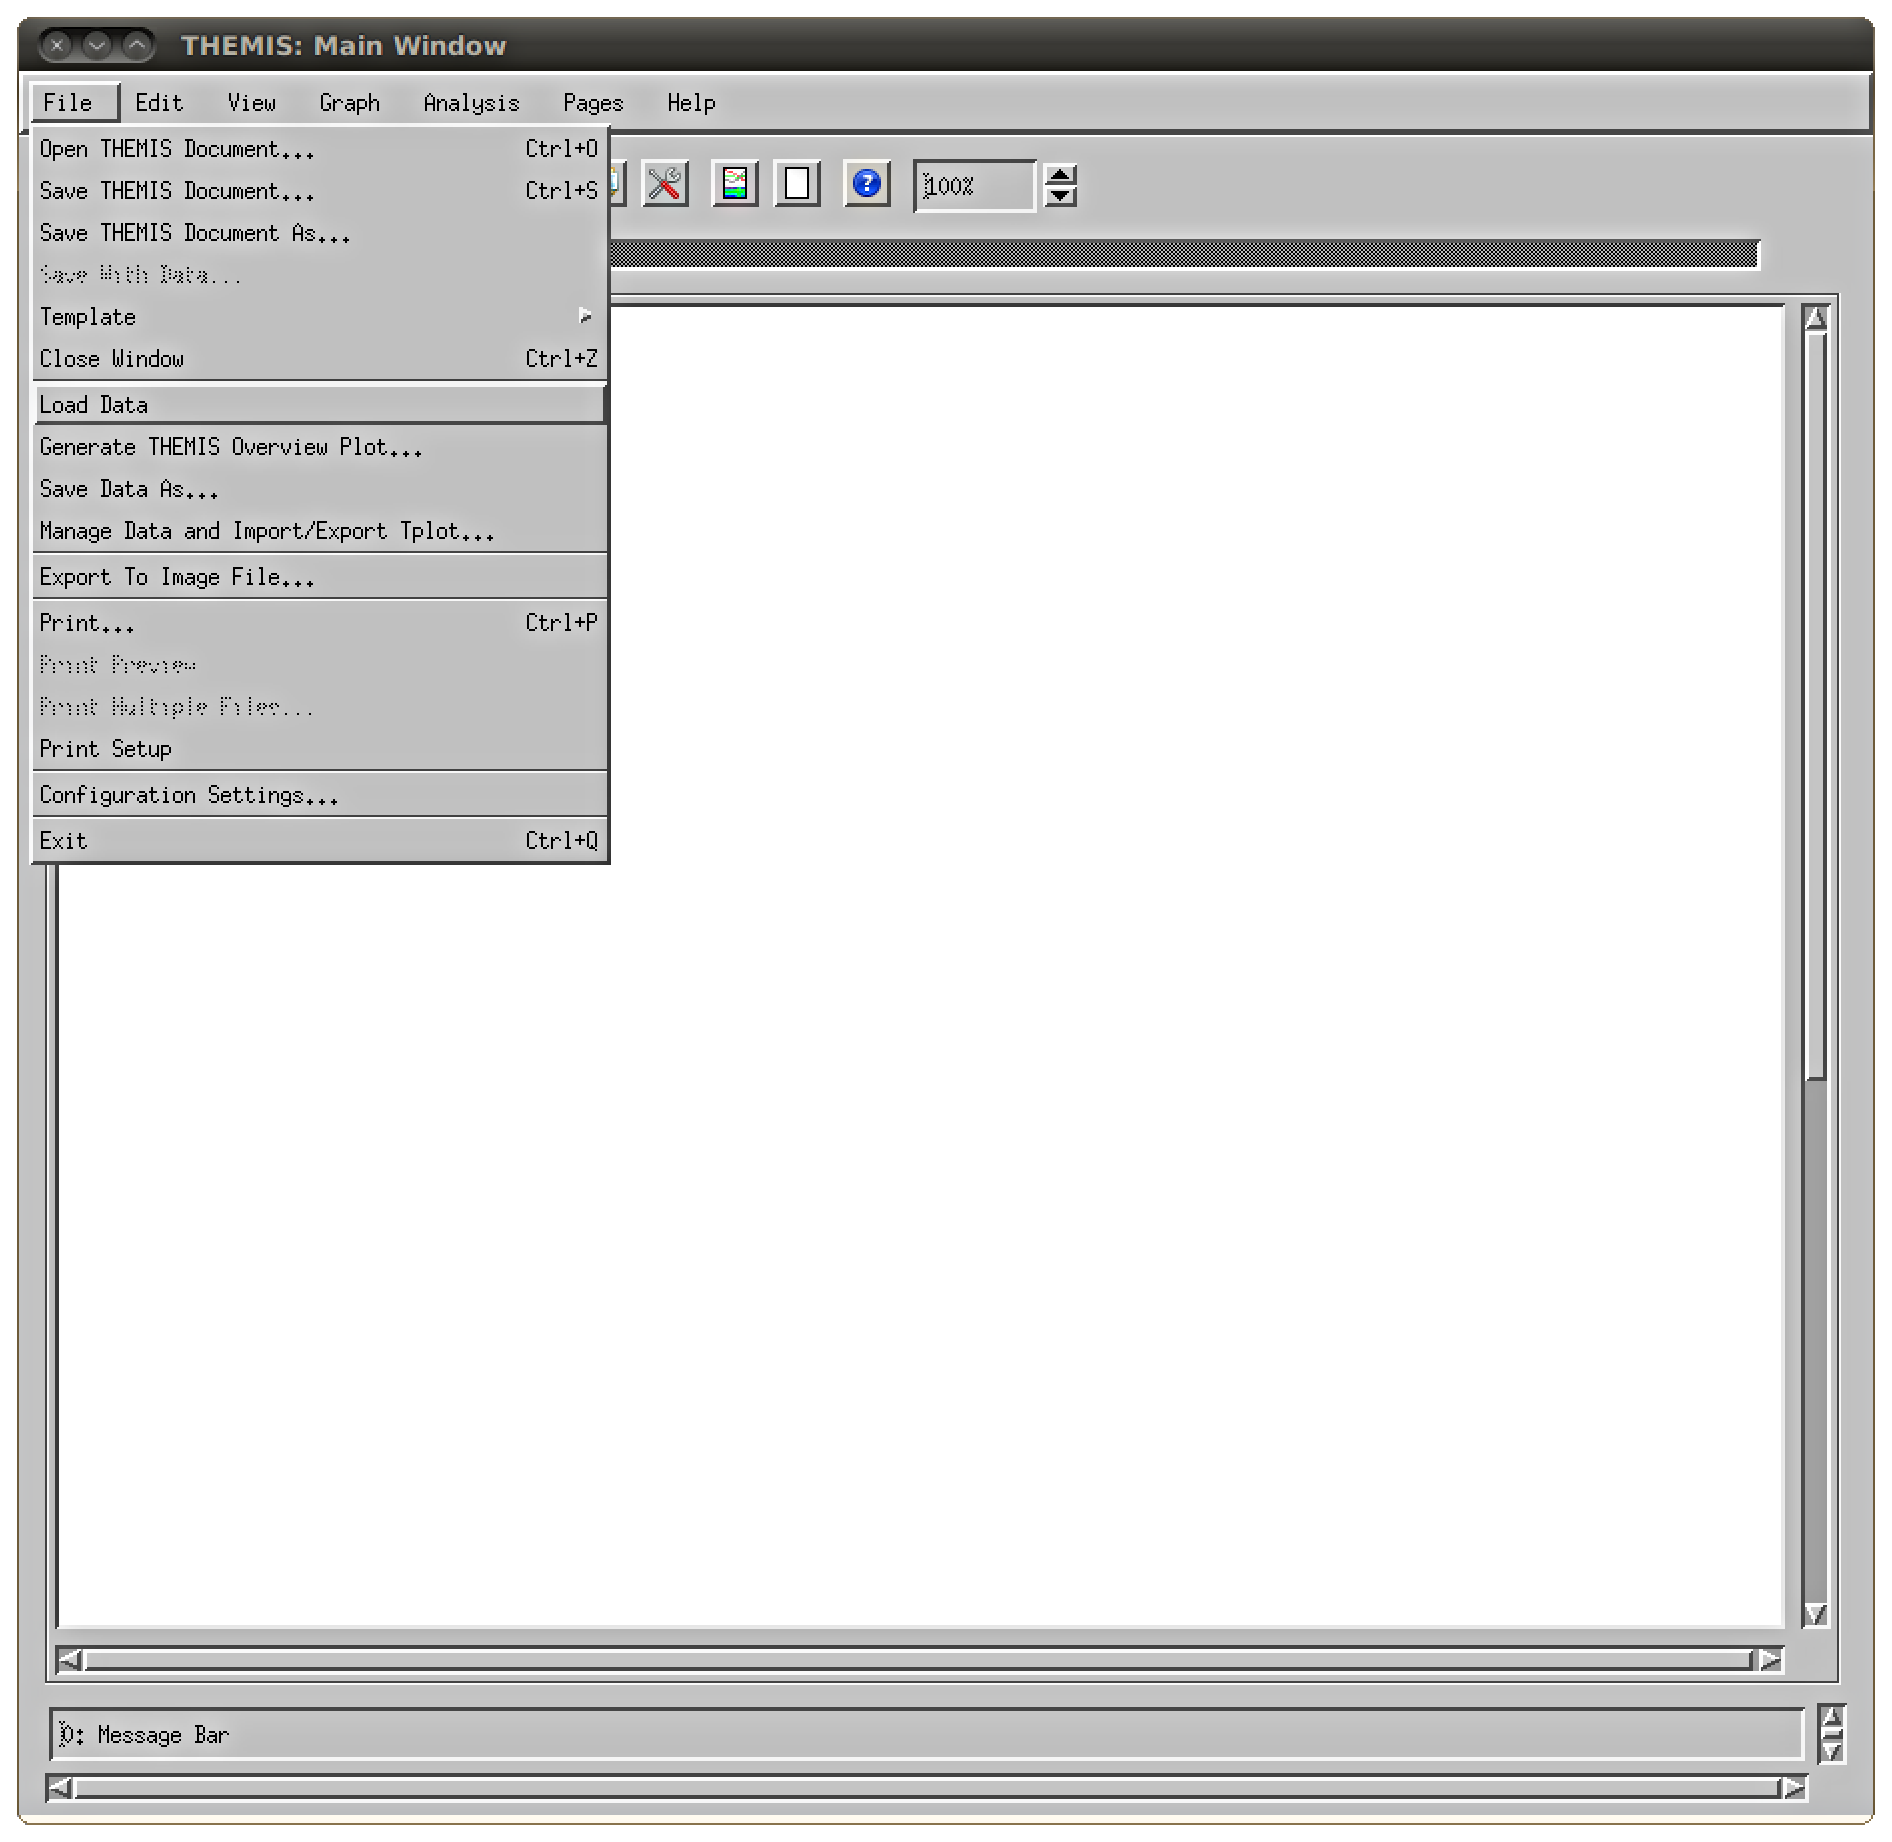
\includegraphics[width=9cm]{images/thm_gui_linux1.eps}
}
\caption{THEMIS: Main Window (Linux)}
\label{thm_gui_linux1.eps}
\end{center}
\end{figure}

\begin{figure}[H]
\begin{center}
\fbox{
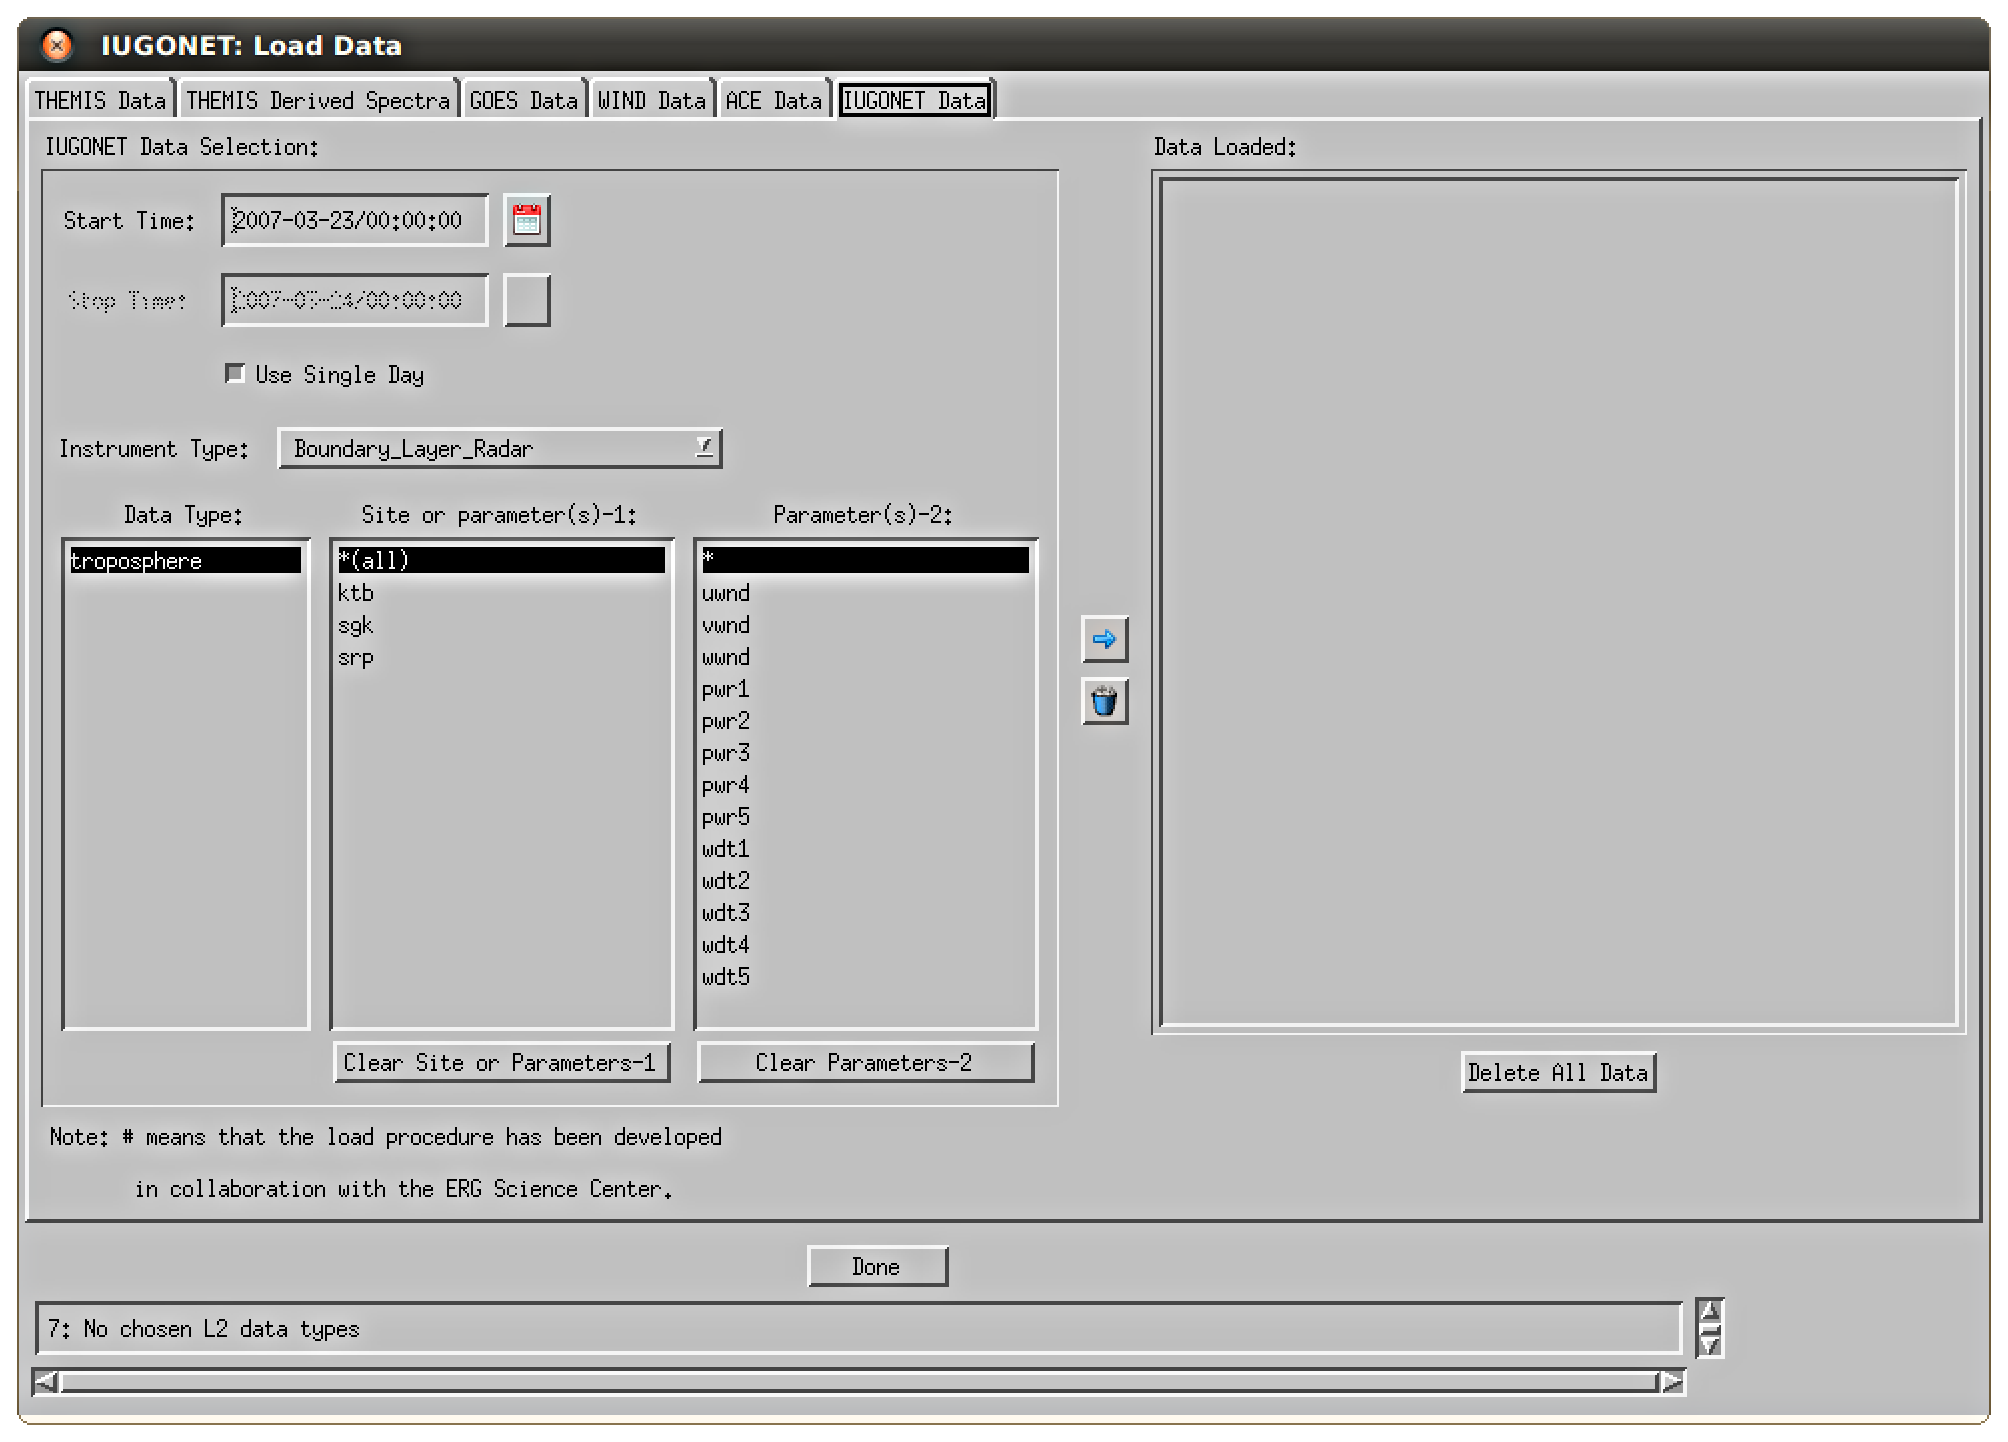
\includegraphics[width=9cm]{images/thm_gui_linux2.eps}
}
\caption{IUGONET: Load Data (Linux)}
\label{thm_gui_linux2.eps}
\end{center}
\end{figure}

\part{TDAS/UDASのインストール(Mac編)}

\chapter{TDASのインストール(Mac編)}
\label{tdas_install_mac}

第\ref{udas_abstract}章の図\ref{udas_deploy}で示したとおり、TDASはIDL上で動作する為、TDASのインストールに先立って、IDLのインストールが必要です。
IDL6.3$\sim$7.1が既にインストールされていることを確認した上で、本章を読み進めて下さい。

\section{TDASのダウンロード}
まずは、tdas\_6\_00.zipをユーザーのホームディレクトリにダウンロードします。
\begin{screen}
\begin{verbatim}
   $ curl http://themis.ssl.berkeley.edu/socware/tdas_6_00/tdas_6_00.zip 
\end{verbatim}
\end{screen}
上記のコマンドでUDASがダウンロード出来ない場合
は、Safari等のブラウザを用いて上記URLにアクセスしてダウンロードして下さい\footnote{ネットワーク環境に
よって、proxyサーバーの設定が必要な場合があります。}。

\section{TDASの展開}
次に、ホームディレクトリ上において、tdas\_6\_00.zipを展開します。
\begin{screen}
\begin{verbatim}
   $ unzip tdas_6_00.zip
\end{verbatim}
\end{screen}
正しく展開出来ていれば、ホームディレクトリにtdas\_6\_00ディレクトリが出来ます。

\section{TDASの環境設定1(IDL\_BASE\_DIRの設定)}

tdas ディレクトリのパスを IDL\_BASE\_DIR という環境変数に設定して、sourceコマンドを実
行します。以下は、tdas を\$\{HOME\}/tdas\_6\_00 に展開した場合を、以下に示します。
\begin{screen}
\begin{verbatim}
$ export IDL_BASE_DIR=${HOME}/tdas_6_00
$ source ${HOME}/tdas_6_00/idl/themis/setup_themis_bash
\end{verbatim}
\end{screen}

\section{TDASの動作確認}
IDLを起動し、thm\_init コマンドを入力し、以下のメッセージが出れば、無事にパスが通っています。
\begin{screen}
\begin{verbatim}
 1 $ idl
 2 IDL> thm_init
 3 THEMIS countdown: xxxxxx xxxxxx xxxx since launch
 4 THEMIS>  
\end{verbatim}
\end{screen}

\section{TDASの環境設定2(Local data directoryとRemote data directoryの設定)}
 TDAS で、Local data directoryとRemote data directoryの設定を行います。
まず始めに、IDLを起動してthm\_gui\_newコマンドを入力します。
\begin{screen}
\begin{verbatim}
 1 $ idl
 2 IDL> thm_gui_new
\end{verbatim}
\end{screen}
次に、\fbox{File}$\rightarrow$\fbox{Configuration Settings...}を選択します。
Configuration Settings... で、THEMIS を選択します。\par
ダウンロードされたTHEMISデータを保存するディレクトリであるLocal data directory
を設定します。ここでは、\$\{HOME\}/data/themisに設定します。\par
最後に、ダウンロード元であるRemote data directoryを設定します。日本国内でTDASを
使用する場合、日本のミラーサイトであり、ネットワーク的に近い
http://themis.stp.isas.jaxa.jp/data/themis/
を設定します。
\fbox{Save}-\fbox{Close}をクリックします。



\chapter{UDASのインストール(Mac編)}
\label{udas_install_mac}

第\ref{udas_abstract}章の図\ref{udas_deploy}に示したとおり、UDASはTDASに依存しています。その為、
UDASのインストールに先立ち、TDASのインストールが必要です。TDASを未だインストールされて
いない場合は、先に第\ref{tdas_install_mac}章をご覧下さい。

\section{UDASのダウンロード}
\begin{screen}
\begin{verbatim}
curl http://www.iugonet.org/software/udas_package_j/udas_1_00_1.zip
\end{verbatim}
\end{screen}
を実行し、udas\_1\_00\_1.zipをダウンロードして下さい。上記のコマンドでUDASがダウンロード出来ない場合
は、Safari等のブラウザを用いて上記URLにアクセスしてダウンロードして下さい\footnote{ネットワーク環境に
よって、proxyサーバーの設定が必要な場合があります。}。

\section{UDASの展開}
前節でダウンロードしたudas\_1\_00\_1.zipを、下記コマンドで展開します。
\begin{screen}
\begin{verbatim}
   $ unzip udas_1_00_1.zip
\end{verbatim}
\end{screen}

\section{UDASの環境設定}

\begin{screen}
\begin{verbatim}
 1 $ echo 'export IDL_PATH=<IDL_DEFAULT>:+/path/to/udas:+/path/to/tdas' 
 2 >> ~/.bashrc
 3 $ source ~/.bashrc
 4 $ idl
 5 IDL>
 6 IDL> print, !path
\end{verbatim}
\end{screen}
紙面の都合上、上記の様に記載しましたが、1, 2行目は途中に改行を入れずに連続して入力して下さい。
1行目において、.bashrcの末尾にIDL\_PATHの設定を追加しています。
2行目において、.bashrcに記述した環境変数IDL\_PATHを反映させます。
3行目においてIDLを起動します。5行目は、1行目において行ったパスの設定が
出来ていることをIDL上において確認します。\par

\section{UDASの動作確認}

ここでは、UDASのGUIの動作確認を行います。まず始めに、コマンドラインから下記コマンドを
入力します。
\begin{screen}
\begin{verbatim}
 1 $ idl
 2 IDL> thm_gui_new
\end{verbatim}
\end{screen}
THEMIS Main Windowが開いた後に、\fbox{File}-\fbox{Load Data}
を選択します(図\ref{thm_gui_mac1.eps})。新しく開いたウィンドウにIUGONETタブが
あれば動作確認終了です(図\ref{thm_gui_mac2.eps})。

\begin{figure}[H]
\begin{center}
\fbox{
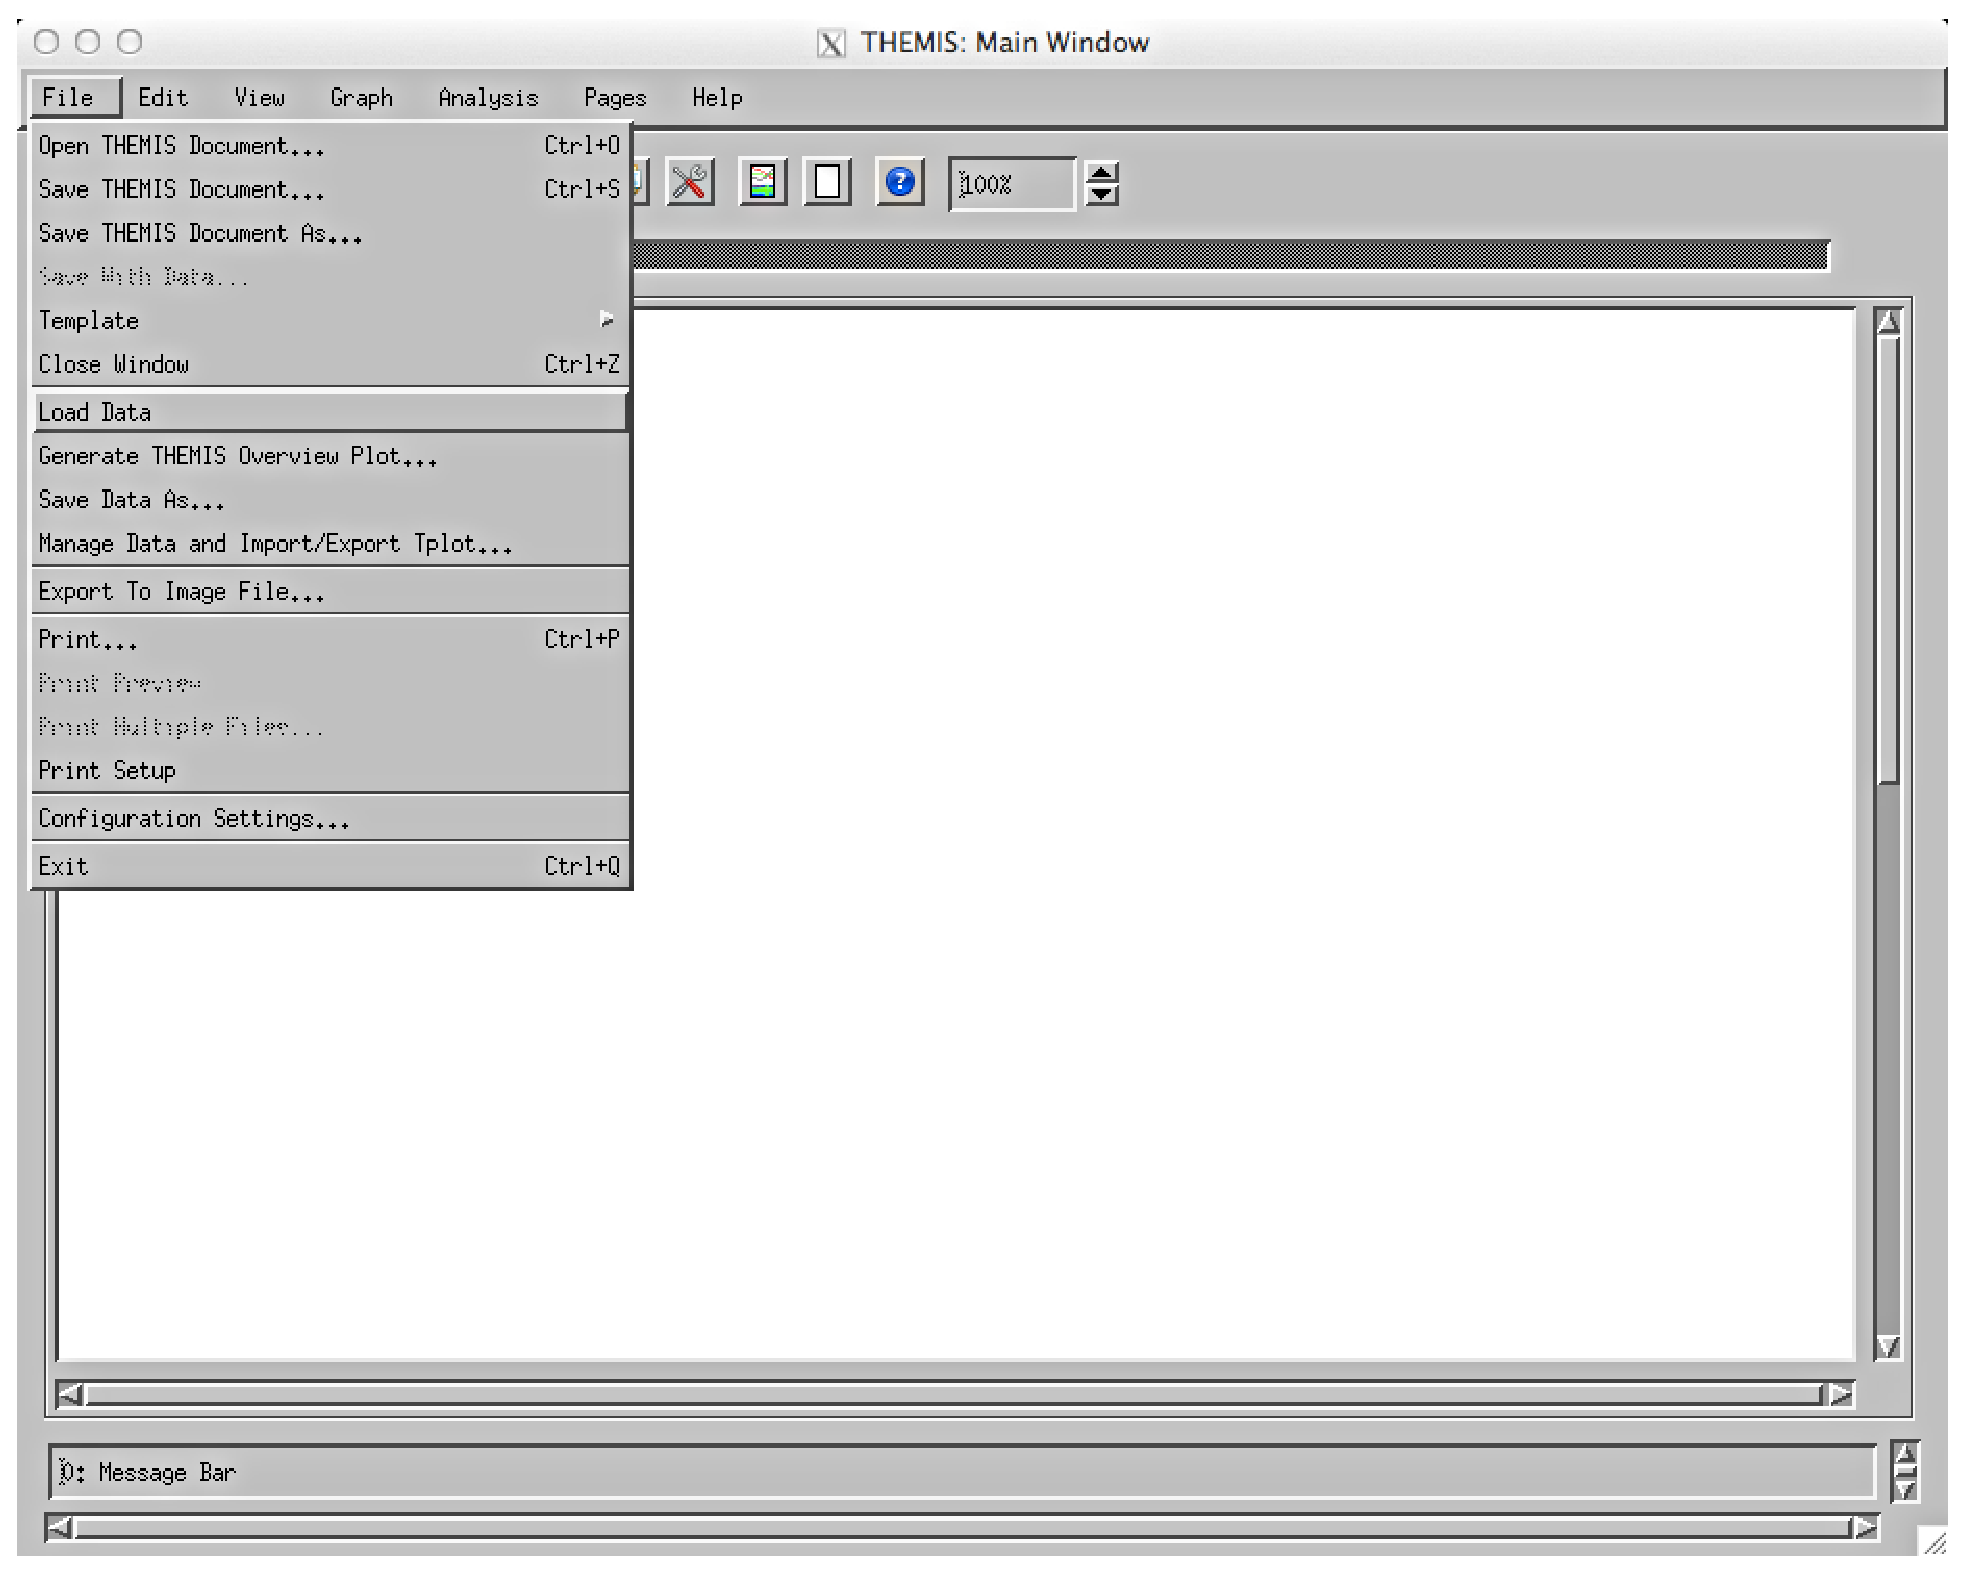
\includegraphics[width=9cm]{images/thm_gui_mac1.eps}
}
\caption{THEMIS: Main Window (Mac)}
\label{thm_gui_mac1.eps}
\end{center}
\end{figure}

\begin{figure}[H]
\begin{center}
\fbox{
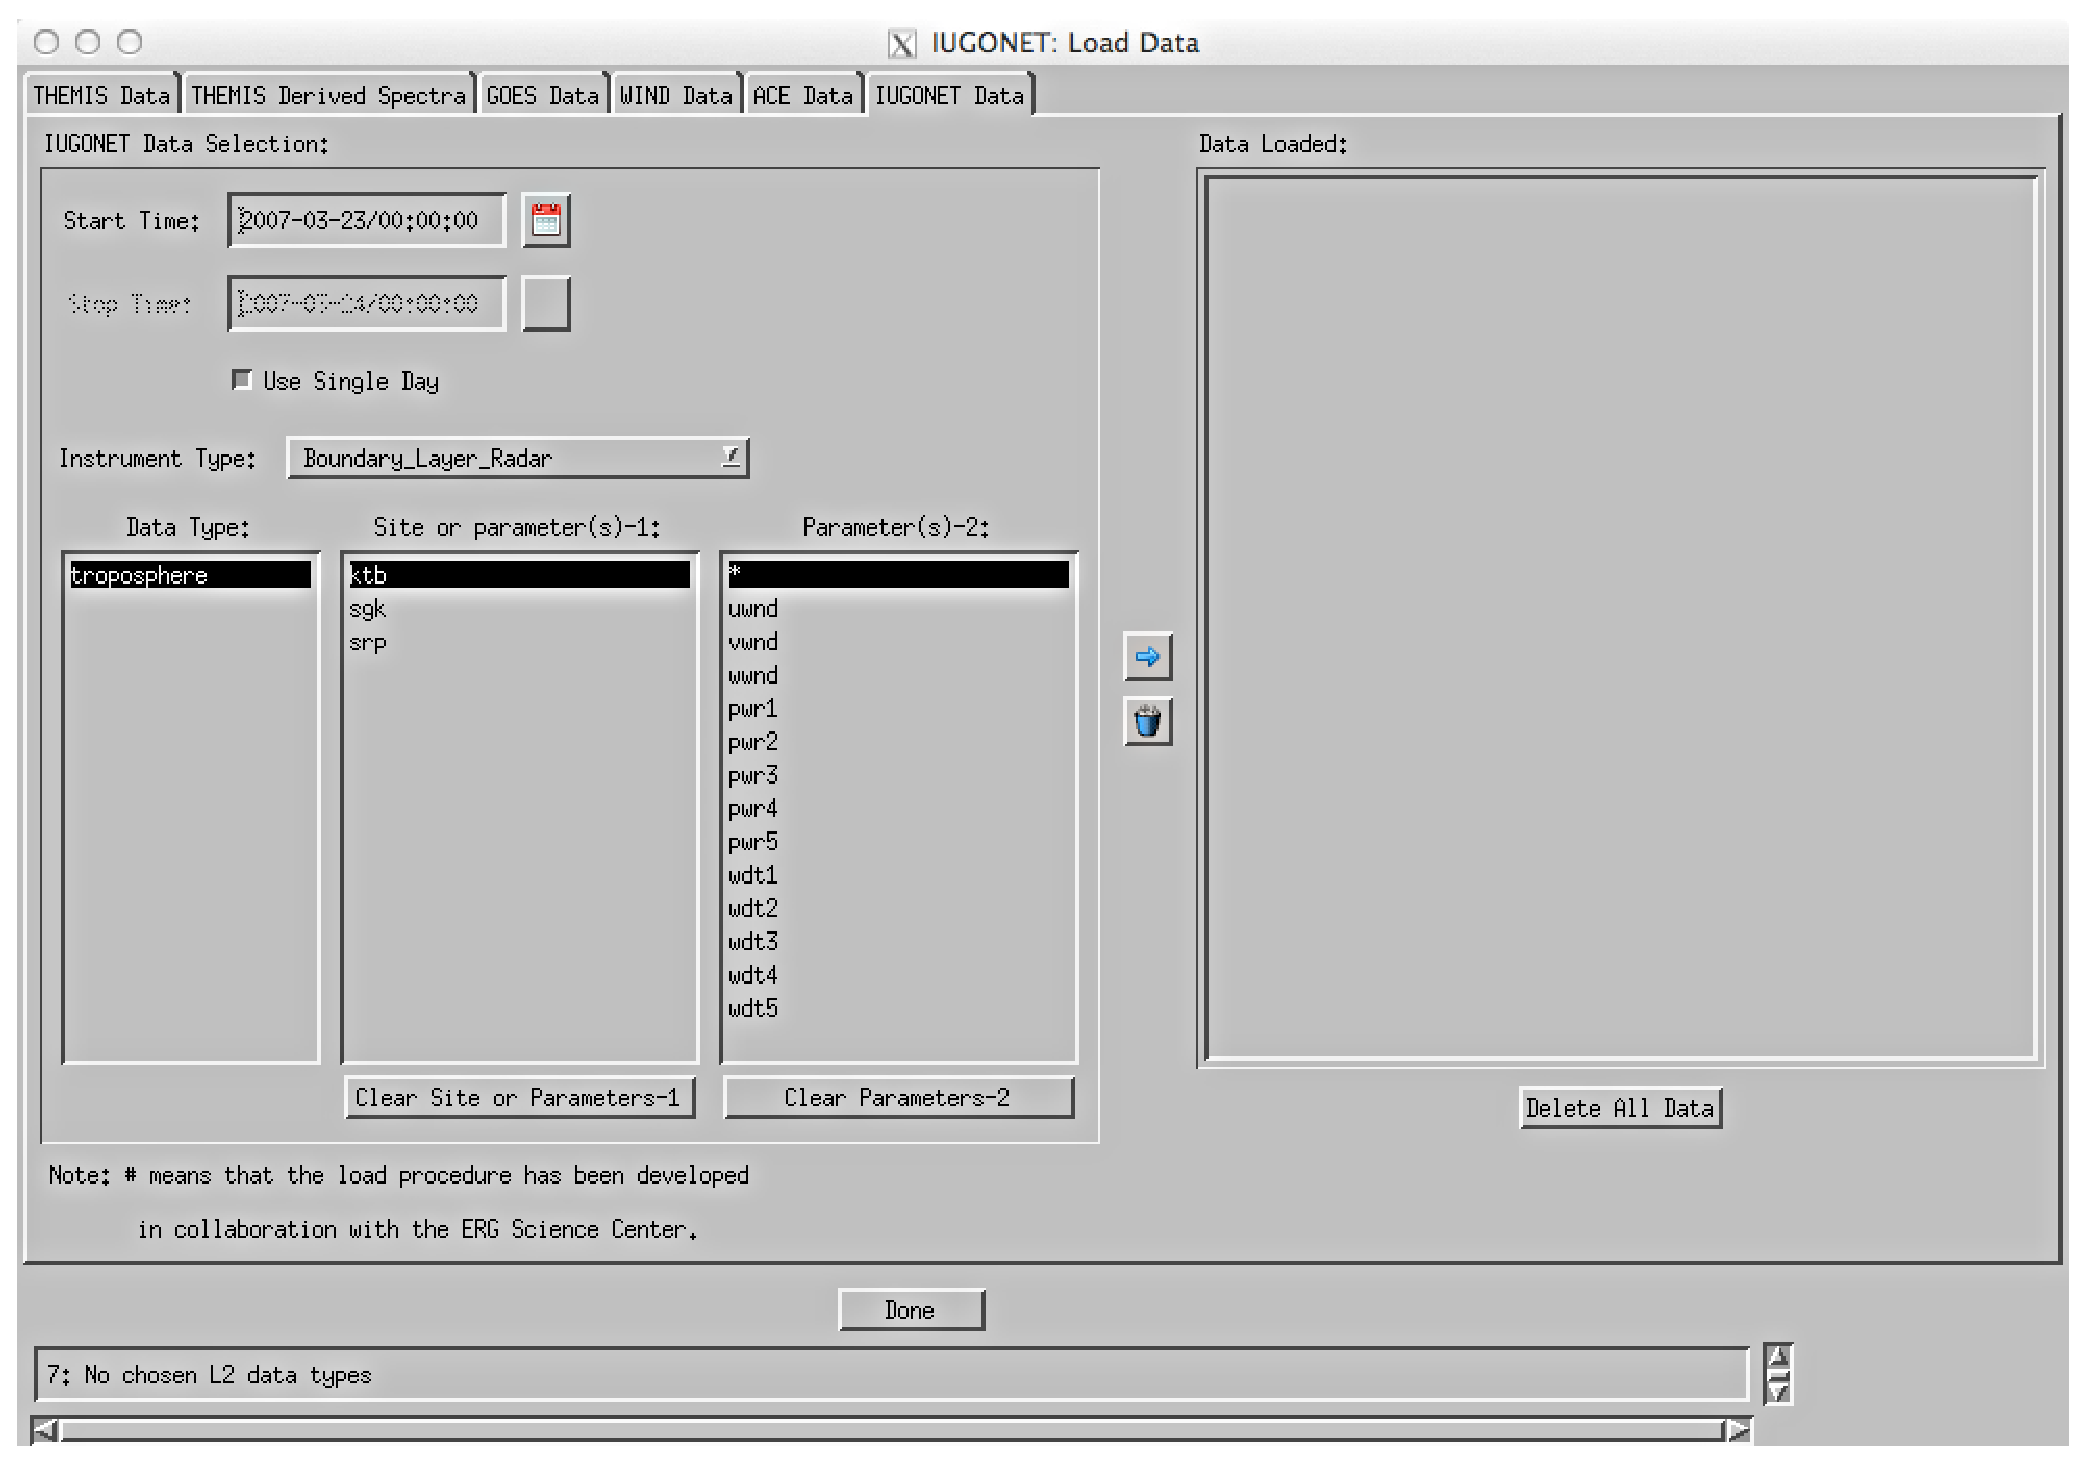
\includegraphics[width=9cm]{images/thm_gui_mac2.eps}
}
\caption{IUGONET: Load Data (Mac)}
\label{thm_gui_mac2.eps}
\end{center}
\end{figure}

\appendix

\chapter{UDASとTDASのバージョン対応表}

表\ref{versions}にUDASとTDASのバージョン対応表を示します。

\begin{table}[H]
\begin{center}
\caption{UDASとTDASの対応バージョン表}
\label{versions}
{\small
\begin{tabular}{c|c}\hline
UDASバージョン & 対応するTDASバージョン \\ \hline
{\color{red}1.00} & {\color{red}v6.00}\\
1.00b4 & v6.00\\
1.00b3 & v6.00\\
1.00b2 & v6.00\\
1.00b1 & v6.00\\
{\color{blue}0.21b1} & {\color{blue}v5.21}\\ \hline
\end{tabular}
}
\end{center}
\end{table}

\begin{thebibliography}{1}
\bibitem[1]{themis} http://themis.ssl.berkeley.edu/software.shtml
\end{thebibliography}

\end{document}
